\documentclass[10pt,twocolumn,letterpaper]{article}
\usepackage{nopageno}

\usepackage{iccv}
\usepackage{times}
\usepackage{epsfig}
% \usepackage{graphicx}
\usepackage{amsmath}
\usepackage{amssymb}
%\usepackage[activate]{pdfcprot}
\usepackage{microtype}
\usepackage{xcolor}
\usepackage[color]{changebar}

% Include other packages here, before hyperref.

% for figures and captions
\usepackage{graphicx}
\usepackage[font=small]{caption}
\usepackage{subcaption}
\graphicspath{{figs/}}

% for putting subcaption labels inside figure to save space
\usepackage{stackengine}
\setlength{\fboxsep}{2pt} 
\newcommand{\inlinelabel}[2]{
    \stackinset{l}{-2pt}{b}{-2pt}{\colorbox{white}{\small(#1)}}{#2}
}

% in-paragraph enumerate
\usepackage{paralist}

% better citing
\usepackage[numbers,square]{natbib}
\setlength{\bibsep}{2pt plus 0.3ex}

% linkcolor should IMHO be switched to black for the submission
\usepackage[pagebackref=false,breaklinks=true,bookmarks=false]{hyperref}
\renewcommand*{\figureautorefname}{Figure}
\hypersetup{%
  pdftitle={anonymous},
  pdfauthor={anonymous},
  bookmarksnumbered,
  pdfstartview={FitH},
  colorlinks,
  citecolor=black,
  filecolor=black,
  linkcolor=black,
  urlcolor=black,
  breaklinks=true,
}

% temporarily uncommented as reverse-search wasn't working for me
% it looks like the hacked-together iccv.sty broke something with the synctex
\iccvfinalcopy % *** Uncomment this line for the final submission

\def\iccvPaperID{1113} % *** Enter the ICCV Paper ID here
\def\httilde{\mbox{\tt\raisebox{-.5ex}{\symbol{126}}}}

\cbcolor{red}
\newcommand{\todo}[1]{\cbstart \textsf{\textbf{\textcolor{red}{[#1]}}} \cbend{}}
\newcommand{\commentE}[1]{\textsf{\textbf{\textcolor{green}{Erroll: #1}}}}
\newcommand{\commentA}[1]{\textsf{\textbf{\textcolor{orange}{Andreas: #1}}}}
\newcommand{\commentT}[1]{\textsf{\textbf{\textcolor{blue}{Tadas: #1}}}}
\newcommand{\commentY}[1]{\textsf{\textbf{\textcolor{purple}{Yusuke: #1}}}}

% create a command to set dataset name
\newcommand{\dataset}{SynthesEyes\xspace}

\usepackage{authblk}

% Pages are numbered in submission mode, and unnumbered in camera-ready
% \ificcvfinal\pagestyle{empty}\fi
\begin{document}

\setlength{\textfloatsep}{\baselineskip + 0.2\baselineskip - 0.2\baselineskip}

%%%%%%%%% TITLE
% \title{Photorealistic Rendering of Face and Eye Regions for Eyelid Detection and Gaze Estimation}
\title{Rendering of Eyes for Eye-Shape Registration and Gaze Estimation}
% Andreas: here we discussed if we want to claim photorealistic since we can't measure it nor know so far if it is really needed. Anyway we need to motivate and show that photorealism is needed. Instead we could use "Accurate"

% Erroll: we'd like to replace "eyelid detection" with something a bit more descriptive, as our system loacalizes them accurately and also gives estimates for iris and therefore eye-centre also. Perhaps "Eye Registration?"
% Andreas: I understand the reasoning and agree. I am not sure, however, if eye registration is an established term, at least I have never heard it before. I would stick to something that people know, maybe landmarks or eye features?
% Andreas: we might want to put "shape model" in the title as well

% \title{Photorealistic Rendering of Human Eyes for Eyelid Detection and Gaze Estimation}
% Andreas; learning-by-synthesis we could also use in the title
% Andreas: what about "Photorealistic Rendering of Face and Eye Images for Large-Scale Eyelid Detection and Gaze Estimation" 

\author{Erroll Wood\textsuperscript{1}, Tadas Baltru\v{s}aitis\textsuperscript{1}, Xucong Zhang\textsuperscript{2}, Yusuke Sugano\textsuperscript{2}, Peter Robinson\textsuperscript{1}, Andreas Bulling\textsuperscript{2}\\
University of Cambridge, United Kingdom
  \texttt{\small\{eww23,tb346,pr10\}@cam.ac.uk} \\
Max Planck Institute for Informatics, Germany
  \texttt{\small\{xczhang,sugano,bulling\}@mpi-inf.mpg.de}
% For a paper whose authors are all at the same institution,
% omit the following lines up until the closing ``}''.
% Additional authors and addresses can be added with ``\and'',
% just like the second author.
% To save space, use either the email address or home page, not both
% \and
% Second Author\\
% Institution2\\
% {\tt\small secondauthor@i2.org}
}

\maketitle
\thispagestyle{empty}

%%%%%%%%% ABSTRACT
\begin{abstract}
%!TEX root = 00_main.tex
Images of the eye are key in several computer vision problems, such as facial feature localization and gaze estimation.
%, iris-biometrics, and deception analysis.
Recent large-scale supervised methods for these problems require time-consuming data collection and manual annotation, which can be unreliable.
%, which is error-prone and slows down progress in these areas.
We propose synthesizing perfectly labelled photo-realistic training data in a fraction of the time.
We used computer graphics techniques to build a collection of dynamic eye-region models from head scan geometry.
%
These were randomly posed to synthesize close-up eye images with a wide range of head poses, gaze directions, and illumination conditions.
%
%\commentA{do we want to sell this also as a dataset? If yes we should characterise it better}
%\commentE{Probably not, as the license doesn't allow "sharing" of data derived from the head scans. "Portfolio work" is fine however, so they shouldn't have issue with using shots of the scan in the paper}
% We validated the usefulness of the dataset on two scenarios: an eye landmark detector and an appearance-based gaze estimator.
% The model is able to simulate the large variability of real eyes, including pupil dilation, eyelid motion and corresponding changes in its shape, as well as iris colour variations.
%dynamic changes in shape
We demonstrate the benefits of our synthesized training data (\dataset) by out-performing state-of-the-art methods for eye-shape registration in the wild, and achieving competitive performance on appearance-based gaze estimation.
% needs reword.
Furthermore, we show that its important to include realistic illumination and shape variation in training data.
\end{abstract}

%%%%%%%%% BODY TEXT

% \commentA{reminder: figures 8 and 10 need reference indices in the legend}
%
% \commentA{figure 11: should read MPIIGaze, i.e. without space}

%!TEX root = 00_main.tex

\section{Introduction}

% \commentA{would be nice to show the process figure as a teaser above abstract as in the disney paper}
% Looks like the template doesn't allow us to do this easily unfortunately :(

Machine learning methods that leverage large amounts of training data currently perform best for many problems in computer vision, such as object detection, scene recognition, or gaze estimation~\cite{zhou2014learning,girshick2014rich,zhang15_cvpr}.
However, capturing or collecting large-scale training data can be time-consuming
%, especially for new areas of research without pre-existing datasets.
and supervised learning methods additionally require accurate ground truth annotation for each image.
This annotation process can be expensive and tedious, and there is no guarantee that human-provided labels will be correct.
Ground truth annotation is particularly challenging and error-prone for learning tasks that require highly fine-grained and accurate labels, such as tracking facial landmarks for facial expression analysis and gaze estimation, or body joints for pose estimation and activity recognition.

\begin{figure}
    \includegraphics[width=\columnwidth]{teaser}
    \caption{At the core of our method is a dynamic eye-region model that allows us to render large numbers of photorealistic eye images as training data for eye region registration and gaze estimation.}
    \label{fig:teaser}
\end{figure}

% \commentE{The further back I look, rendering RGB training images does go back into the past for pose-estimation at least, though none of it was ``photorealistic''}
To address these problems, researchers have employed \emph{learning-by-synthesis} techniques to generate large amounts training data with computer graphics.
The advantages of this approach are that both data collection and annotation require little human labour and image synthesis can be geared to specific application scenarios.
Perhaps the best known example is by \citet{shotton2013real}, who synthesized a large and varied depth-image dataset for training a real-time pose-estimator.

The eyes and their movements are important for a range of applications including gaze-based human-computer interaction~\cite{majaranta14_apc}, visual behaviour monitoring~\cite{bulling13_chi,bulling11_pami}, and -- more recently -- computer vision tasks, such as object recognition and detection~\cite{yun2013studying,papadopoulos2014training,karthikeyan2013and}.
The eye-region is particularly difficult to model accurately given the dynamic shape changes it undergoes with facial motion and eyeball rotation, and the complex material structure of the eyeball itself.
For this reason, a recent learning-by-synthesis work for gaze estimation employed only fundamental computer graphics techniques -- rendering low-resolution meshes without allowing lighting variation or accounting for the varying material properties of the face \citet{sugano2014learning}.
In addition, their model was not fully controllable and the synthesized dataset contained only gaze labels, limiting its usefulness for other computer vision problems, such as facial landmark registration.
\commentA{what about Leszeks work? should also fit in here, right?}

% \commentA{we can also remove these last references if we have to save space}
% Recent work by \citet{sugano2014learning} demonstrated the benefits of learning-by-synthesis for appearance-based gaze estimation, but employed only fundamental computer graphics techniques for synthesising low-resolution meshes that did not account for lighting variation.

% It is for this reason that previous work on rendering photorealistic images of the eye and eye-region is relatively sparse~\cite{ActiBlizEyes,berard2014highquality}.
% \commentY{What does this "sparsity" mean? And again, I think having 10 different models is a little to weak to say that it can handle "significant variation in facial shape and texture across different people" in the context of face/eye research.}

% \commentA{we also need to motivate why high quality renderings are needed, i.e. why it's worthwhile to put so much effort into the model. And later we can hopefully also show that it pays off to do so...}

% Andreas: we need some transition to eyeballs here, e.g. eyeball rendering is particularly challenging and interesting because of the many muscles involved, the large number of appearance details around and in the eye etc.
% essentially motivate that this hasn't been done before and is a very interesting area of research

%Synthesising training data is not novel in itself -- previous work has ... Our novel approach 

\begin{figure*}
    \centering
    \begin{subfigure}[t]{0.195\textwidth}
        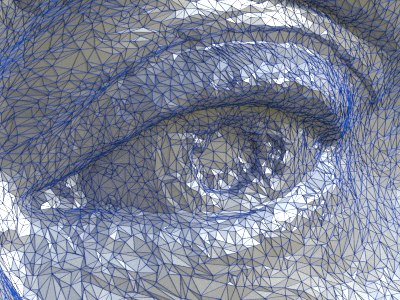
\includegraphics[width=\textwidth]{process_f02_01}
        \caption{Original 3D head scan data: 1.4 million polys}
        \label{fig:process_original_scan}
    \end{subfigure}
    \hfill
    \begin{subfigure}[t]{0.195\textwidth}
        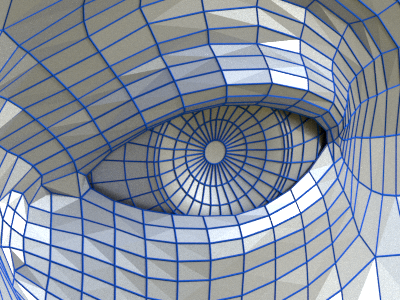
\includegraphics[width=\textwidth]{process_f02_02}
        \caption{Retopologized head model: 9 thousand polys}
        \label{fig:process_retopo}
    \end{subfigure}
    \hfill
    \begin{subfigure}[t]{0.195\textwidth}
        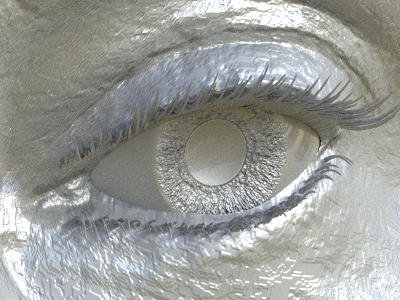
\includegraphics[width=\textwidth]{process_f02_03}
        \caption{Surface detail is stored in displacement maps}
        \label{fig:process_displaced_subdiv}
    \end{subfigure}
    \hfill
    \begin{subfigure}[t]{0.195\textwidth}
        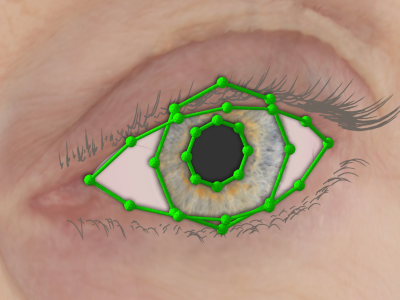
\includegraphics[width=\textwidth]{process_f02_04}
        \caption{3D iris and eyelid landmarks are annotated}
    \end{subfigure}
    \hfill
    \begin{subfigure}[t]{0.195\textwidth}
        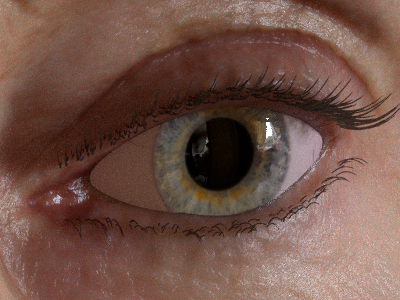
\includegraphics[width=\textwidth]{process_f02_05}
        \caption{The final render}
    \end{subfigure}
    \caption{Model preparation process}
    \label{fig:process}
\end{figure*}

We present a novel method for realistic rendering face and eye images at a large scale using a collection of dynamic and controllable eye-region models.
In contrast to previous works, we provide a comprehensive and detailed description of the model preparation process and rendering pipeline (see~\autoref{fig:process} for an overview of the model preparation process and~\autoref{fig:eye_model} for the eye model used).
We then present and evaluate two separate systems trained on the resulting data (\emph{\dataset}): a novel eye-region specific deformable model and an appearance-based gaze estimator.
These systems are case studies that show how we leverage the controllability made possible by our model to easily and quickly generate high-quality training datasets.
Please note that we picked these two examples for illustration purposes only.
Our model is not limited to these computer vision tasks per se but potentially applicable to other tasks that require \commentA{insert requirements that our model covers}.
To ensure reproducibility and stimulate research in this area we will make the eyeball model and generated training sets publicly available at time of publication.

The specific contributions of this work are threefold.
First, we present our dynamic eye-region model that uses multiple parts and blend shapes to model the continuous degrees of shape change and deformation exhibited by the eye.
We further describe in detail our novel but straight-forward techniques for generating large degrees of realistic lighting variation in synthesized training data using image-based-lighting.
We show that \commentA{insert key appearance-based gaze estimation result here}
We finally present eye-region registration as a novel application of learning-by-synthesis and demonstrate that \commentA{insert key result here}
%!TEX root = 00_main.tex

\section{Related Work}

Our work is related to previous works on 1) learning using synthetic data and 2) computational modelling of the eyes.

\subsection{Learning Using Synthetic Data}

Learning-based approaches have been recognised as a promising solution for various computer vision tasks
% the gap between training and test data still causes practical issues.
but it remains challenging for such approaches to handle unknown test data and their performances often depends on how well the test data distribution is covered by the training data.
Given that recordings of training data that covers the whole variation of potential test data is challenging,
%One solution is to use training data that covers the whole variation of potential test data but it is not always possible to obtain real training data in this manner.
the use of purely synthetic training data has been considered as a promising solution.
Previous works demonstrated that synthetic training data is beneficial for tasks such as body pose estimation~\cite{shakhnarovich2003fast,okada2008relevant,shotton2013real}, head pose estimation~\cite{fanelli2011real}, and object detection/recognition~\cite{yu2010improving,liebelt2010multiview,jaderberg2014synthetic}.
These works used 3D models, from a single 3D CAD object to deformable human body shape, to synthesise large amounts of training images.
% \commentY{CAD-based multi-view object recognition has a lot of works, though I don't think we need to cite them all}

% \commentY{In some sense this is an important reference for our story}
As discussed by \citet{kaneva2011evaluation}, one of the most important factors to consider is the realism of synthesised training images.
If the object of interest is highly complex, like the human eye, it is not clear whether we can rely on overly-simplistic object models.
\citet{zhang15_cvpr} revealed that estimation accuracy significantly drops when the test data is obtained from a different environment.
Similarly to facial expression recognition~\cite{stratou2011effect}, illumination effects are a critical factor for computer vision, and the change of viewpoints is not enough to cover the test data variability.
% \commentY{Is the following line correct? I thought they are just evaluating robustness of their approach against these factors}
% \citet{zface} varied ambient and directional lighting conditions during synthesis to achieve illumination invariance.
% \commentY{this line should be adjusted according to the result}
In contrast, our model allows the synthesis of realistic lighting effects -- an important degree of variation crucial for performance improvements in eye-shape registration.

% \commentY{reality and controllability should be both important, while currently the story focuses on the reality side. but this point is rather related to the next section (Computer Generated Eyes) maybe?}
Most similar to this work, \citet{sugano2014learning} used 3D reconstructions of eye regions to synthesise multi-view training data for appearance-based gaze estimation.
One limitation of that work is that they do not provide a parametric model.
Their data is essentially a set of rigid and low-resolution 3D models of eye regions with ground-truth gaze directions, and hence cannot be easily applied to different tasks.
The scope of learning-by-synthesis with a realistic eye model is not limited to appearance-based gaze estimation; the model can be also applied to other problems, e.g. eye shape registration.
Since our model is fully synthetic, it can be used to synthesise close-up eye images with ground-truth eye landmark positions.
This enables us to address eye shape registration via learning-by-synthesis for the first time.

%\cite{okada2008relevant}, \cite{shakhnarovich2003fast} -- both rendered RGB training images with poser for pose recognition
%\cite{fanelli2011real} -- train head pose estimator on only synthetic depth data.
%\cite{stratou2011effect} -- relit 3d face scans to study the effect of illumination on automatic expression recognition.
%\cite{sugano2014learning} -- learning by synthesis for 3D gaze estimation

%\commentY{(As one of the authors) I think this approach is in a little different context and we don't necessarily need to mention here:} \cite{lu2012head}

\subsection{Computational Modelling of the Eyes}

% \commentA{first paragraph: other body parts, then second paragraph: In contrast, the problem of modelling the human eye has received considerably less attention.}

% \cite{alabort2014statistically} -- trained a detailed deformable eye region model on in-the-wild images.

The eyeballs are complex organs comprised of multiple layers of tissue, each with different reflectance properties and levels of transparency.
Fortunately, given that realistic eyes are important for many areas of computing, there is already a large body of previous work on modelling and rendering eyes (see~\cite{ruhland2014look} for a recent survey).

% As we spend so much time looking at eyes, mistakes in their appearance can cause a CG face to appear unfamiliar.

Eyes are important for the entertainment industry, who want to model them with potentially dramatic appearance (e.g. crying).
\mbox{\citet{ActiBlizEyes}} recently developed techniques for real-time modelling of eye wetness, refraction, and ambient occlusion in a standard rasterisation pipeline for video games.
\citet{berard2014highquality} represents the state-of-the-art in computer representation of eyes.
They used a hybrid reconstruction method to capture both transparent corneal surface and diffuse sclera separately and recorded deformations of the eyeball's interior structures.
However, this required imaging at a close range with specialist hardware.

Aside from visual effects, previous work has used CG models to examine the eye from a medical perspective.
\citet{sagar1994virtual} built a virtual environment of the eye and surrounding face for mechanically simulating surgery with finite element analysis.
\citet{priamikov14_openeyesim} built a 3D biomechanical model of the eye and its interior muscles to understand the underlying problems of visual perception and motor control.
CG eyes have also been used to evaluate geometric gaze estimation algorithms, allowing individual parts of an eye tracking system to be evaluated separately~\cite{bohme2008software,swirski2014rendering}.
\citet{swirski2014rendering} used a rigged head model and reduced eyeball model to render ground truth images for pupil tracking algorithms.

% reword
% The facial region around the eye is also important. There is a vast amount of research on animating and rendering the face ... \cite{orvalho2012facial}

% and the level of detail was deemed unnecessary for our purposes.

% \subsection{Gaze estimation}

% \cite{xiong2014gaze} -- regression with features of 3d pupil centers and eye-contours (the eyelids) for gaze estimation.  Use multiple cameras and IR lights.

%!TEX root = 00_main.tex

\begin{figure*}
    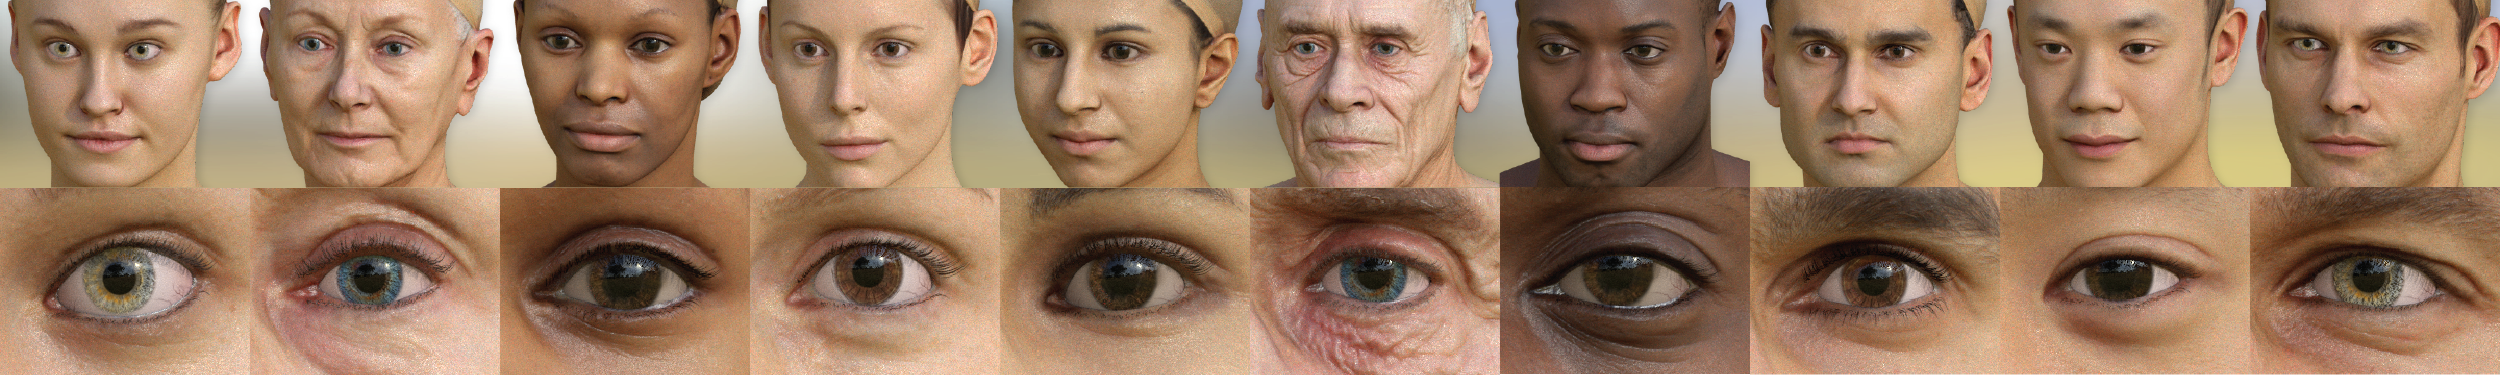
\includegraphics[width=\textwidth]{model_suite}
    \caption{Set of head models and corresponding close-ups of the eye regions used in our method. The set includes 10 different head models of both genders that cover a range of ethnicities and ages.}
    \label{fig:model_suite}
\end{figure*}

\section{Our Dynamic Eye-Region Model}


\begin{figure*}
    \centering
    \begin{subfigure}[t]{0.195\textwidth}
        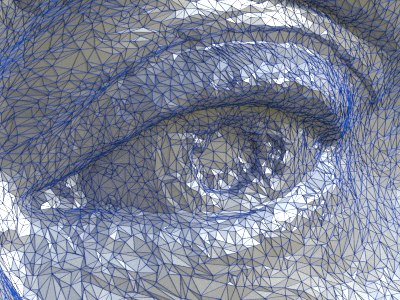
\includegraphics[width=\textwidth]{process_f02_01}
        \caption{Original 3D head scan data: 1.4 million polys}
        \label{fig:process_original_scan}
    \end{subfigure}
    \hfill
    \begin{subfigure}[t]{0.195\textwidth}
        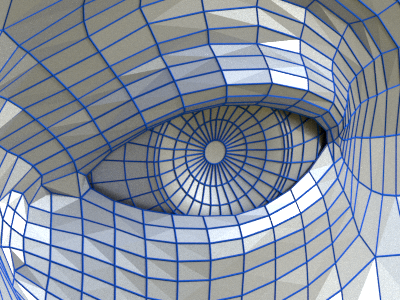
\includegraphics[width=\textwidth]{process_f02_02}
        \caption{Retopologized head model: 9 thousand polys}
        \label{fig:process_retopo}
    \end{subfigure}
    \hfill
    \begin{subfigure}[t]{0.195\textwidth}
        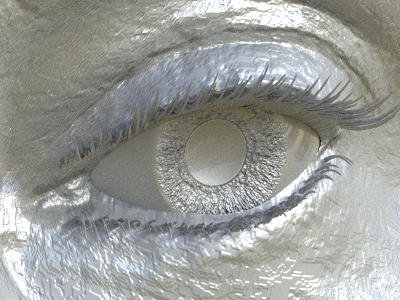
\includegraphics[width=\textwidth]{process_f02_03}
        \caption{Surface detail is stored in displacement maps}
        \label{fig:process_displaced_subdiv}
    \end{subfigure}
    \hfill
    \begin{subfigure}[t]{0.195\textwidth}
        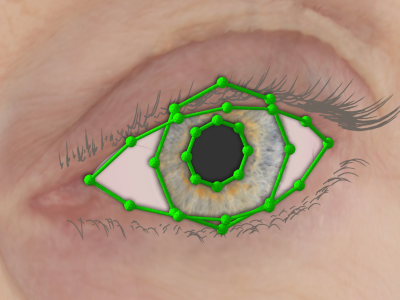
\includegraphics[width=\textwidth]{process_f02_04}
        \caption{3D iris and eyelid landmarks are annotated}
    \end{subfigure}
    \hfill
    \begin{subfigure}[t]{0.195\textwidth}
        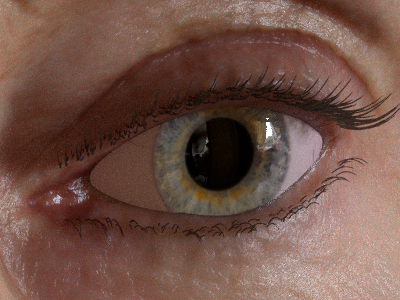
\includegraphics[width=\textwidth]{process_f02_05}
        \caption{The final render}
    \end{subfigure}
    \caption{Model preparation process}
    \label{fig:process}
\end{figure*}

We developed a realistic dynamic eye-region model which can be randomly posed to generate fully labeled training images.
% For a set of training images to be useful, it should be large, representitive of real-world variety, and cleanly labelled.
For training data to be useful, it should be representitive of real-world variety.
Our goal therefore was to model the continuous changes in appearance that the face and eyes undergo following eye movement, so they are accurately represented in close-up synthetic eye images.
This is more challenging than simply rendering a collection of static models, as dynamic geometry must be correctly topologized and rigged to be able to deform continuously.
% this sentence is a bit clunky
Appearance-wise, the eye-region is one of the most complex areas of the whole body. The eyelids, upper-cheek, and eye-ball can all move independently, and feature a range of reflectance properties and small-scale details.
%
In this section we first present our anatomically inspired computer graphics eyeball model, and then explain our procedure for converting a collection of static 3D head scans into dynamic eye-region models that can adopt a wide range of realistic poses, and are suitable for labelled data generation.
%\commentA{I think it would be good to first describe in 1-2 paragraphs what the particular challenges of modelling eye shape, dynamics etc. are. This gives better context for the method description that follows and hopefully also underlines that this is a non-trivial task and the work therefore a significant step forward.}

%\todo{past tense}
%\commentA{we have to explain what makes the model dynamic}
%\commentA{could be nice to show existing renderings and ours side by side, e.g. Leszeks and others (if any)}

\subsection{Simplified Eyeball Model}
\label{subsec:eyeball_model}

\begin{figure}
    \captionsetup[subfigure]{labelformat=empty} % stop subcaption writing "(a)""
    \captionsetup{subrefformat=parens} % add parentheses to \subref
    \begin{subfigure}[t]{0.33\columnwidth}
        \inlinelabel{a}{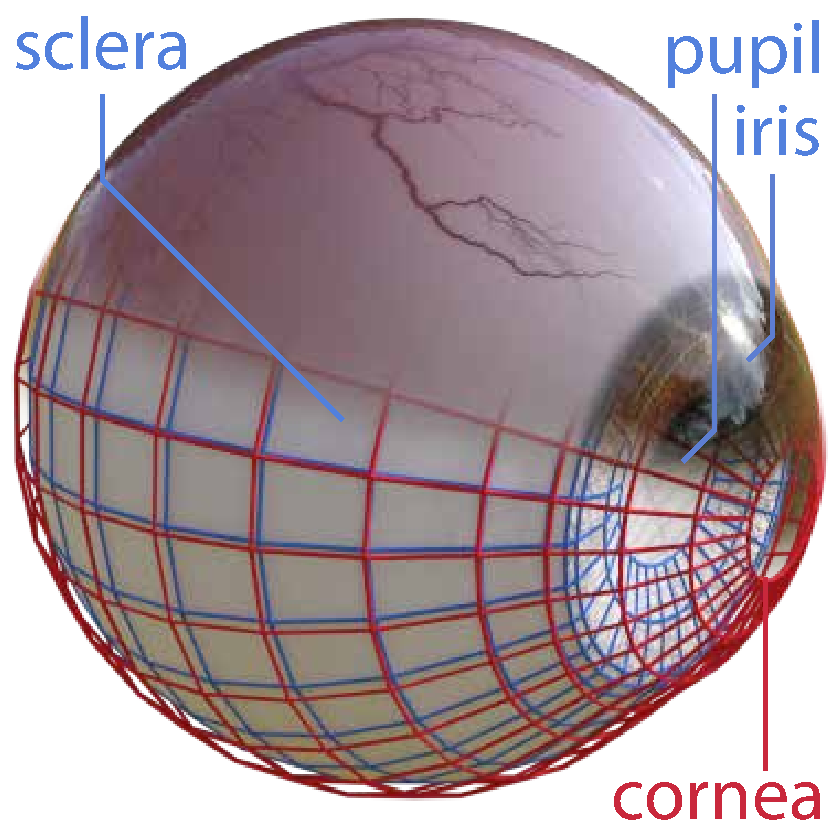
\includegraphics[width=\textwidth]{eye_model}}
        \caption{}\label{fig:eye_model_parts}
    \end{subfigure}
    \hfill
    \begin{subfigure}[t]{0.65\columnwidth}
        \inlinelabel{b}{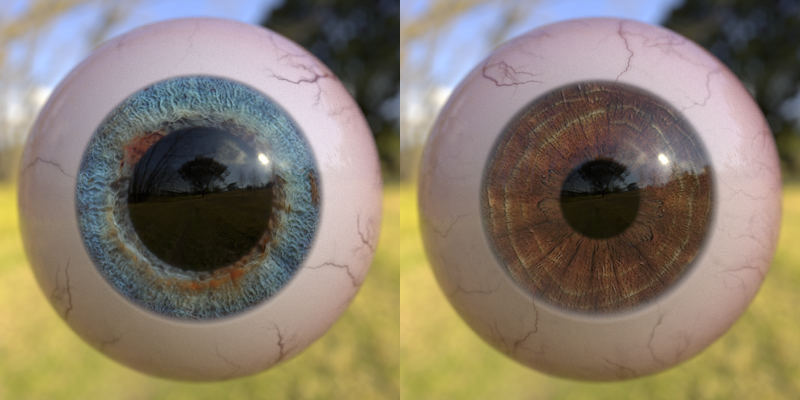
\includegraphics[width=\textwidth]{eye_examples}}
        \caption{}\label{fig:eye_model_images}
    \end{subfigure}
    \par\vspace{-28pt}
    \caption{Our eye model includes the sclera, pupil, iris, and cornea \subref{fig:eye_model_parts} and can exhibit realistic variation in both shape (pupillary dilation) and texture (iris color, scleral veins) \subref{fig:eye_model_images}.}
    \label{fig:eye_model}
\end{figure}

% It is important to accurately model reflections and refractions in the eye as they can lead to specular highlights -- these common eye-region image features are often used by eye-tracking algorithms, or can confound approaches that are not robust.

As shown in \autoref{fig:eye_model_parts}, our eye model consists of two parts.
The outer part (red wireframe) approximates the eye's overall shape with two spheres ($r_1\!=\!12\textrm{mm}, r_2\!=\!8\textrm{mm}$ \cite{ruhland2014look}), the latter representing the corneal bulge.
To avoid a discontinuous seam between spheres, their meshes were joined, and the vertices along the seam where smoothed to minimize differences in face-angle.
% \commentA{how joined and smoothed?} Erroll - Maybe needs rewording. Perhaps i'll just put a citation for the smoothing operation? I don't particularly want to describe it
This outer part is transparent, refractive ($n\!=\!1.376$), and partially reflective.
The sclera's bumpy surface is modelled with smoothed solid noise functions, and applied using a \emph{displacement map} -- a 2D scalar function that shifts a surface in the direction of its normal \cite{lee2000displaced}.
The inner part (blue wireframe) is a flattened sphere  -- the planar end represents the iris and pupil, and the rest represents the sclera, the white of the eye.
There is a $0.5\textrm{mm}$ gap between the two parts which accounts for the thickness of the cornea.
% \commentE{compare with recent Disney work}

Eyes exhibit variation in both shape (pupillary dilation) and texture (iris color and scleral veins).
To model shape variation we use \emph{blend shapes} -- an animation technique where several different poses are created for the same topological mesh, and then interpolated between\cite{orvalho2012facial}. 
We created blend shapes for dilated and constricted pupils, as well as large and small irises to account for a small amount ($10\%$) of variation in iris size.
% Maybe try to explain blend shapes better
% Blend shapes are localized so can be mixed, so we can easily model an eye with a small pupil, and a large iris.
We vary the texture of the eye by randomly compositing images in three separate layers:
\begin{inparaenum}[\itshape i\upshape)]
\item a \emph{sclera} tint layer (white, pink, or yellow);
\item an \emph{iris} layer with four different photo-textures (amber, blue, brown, grey); and
\item a \emph{veins} layer (blood-shot or clear).
\end{inparaenum}
% We matched the sclera tint to each separate face model but uniformably randomly varied iris color.
% Maybe move to related work?
% Previous research on iris-synthesis \commentE{cite} would have allowed continually different iris textures, but we decided this added complexity would not make a worthwhile improvement in overall appearance variation, especially when rendered at lower resolutions.

\subsection{3D Head Scan Acquisition}
\label{sec:eye_region_geom_prep}

For an eye-region rendering to be realistic, it must also feature realistic nearby face detail.
While previous approaches used lifelike artist-created models, for example~\cite{swirski2014rendering}, we instead rely on high-quality head scans captured by a professional photogrammetry studio (10K diffuse color textures, 0.1mm resolution geometry)\footnote{Ten24 3D Scan Store -- \url{http://www.3dscanstore.com/}}.
%\cite{Ten24}.
%\commentA{link or even better reference if available}
%Nowadays it is possible to purchase such scans online (from $\sim\!\$15$/scan)
%or use free or commercial photogrammetry software to generate facial geometry models in-house.
Facial appearance around the eye varies dramatically between people as a result of different eye-shapes (e.g. round vs hooded), orbital bone structure (e.g. deep-set vs protruding), and flesh detail (wrinkled vs flat). Therefore our head models (see \autoref{fig:model_suite}) cover both genders with a variety of ethnicities and ages.

\subsection{Eye-Region Geometry Preparation}

As can be seen in \autoref{fig:process_original_scan}, the cornea has been incorrectly reconstructed by the optical scanning process.
This is because transparent surfaces are not directly visible, so cannot be reconstructed in the same way as diffuse surfaces, such as skin.
% Recent work used a hybrid reconstruction method to reconstruct the corneal surface separately, but requires additional hardware \cite{berard2014highquality} -- this level of detail was deemed unnecessary for our purposes.
We wanted images representing a wide range of eye-gaze directions, so we needed to be able to pose the eyeball separately from the face geometry.
We therefore removed the scanned eyeball from the mesh, and placed our own eyeball approximation in its place.
\commentY{I feel this part should be explained beforehand,  i.e., we should first explain why take this approach combining eye model and face scan}

While the original head scan geometry is suitable for being rendered as a static model, its topology cannot easily represent dynamic changes in eye-region shape.
Vertical saccades are always accompanied by eyelid motion \cite{liversedge2011oxford}, so we needed to be able to pose the eyelids according to the gaze vector.
When preparing a mesh for facial animation, edge loops should flow along and around the natural contours of facial muscles.
This leads to a more efficient (low-resolution) geometric representation of the face, and more realistic animation as mesh deformation matches that of actual skin tissue and muscles.

% Maybe: \commentE{Reference some other options, e.g automatic methods in research}

\commentY{I feel this paragraph requires knowledge on both computer graphics and eye movement researches, not easy for ordinary CV readers}
We therefore \emph{retopologized} the face geometry into a more optimal form using a commercial semi-automatic system \cite{ZRemesher}.
% Erroll: changed just the sentence below to present tense. As the model still exists, perhaps the tense should be present? Not sure.
As can be seen in \autoref{fig:process_retopo}, edge loops now follow the \emph{Orbicularis Oculi} muscle, allowing for realistic eye-region deformations.
This retopologized low-poly mesh has now lost the detail of the original scan and has visible sharp edges.
We therefore used it as a displaced subdivision surface \cite{lee2000displaced} with displacement map computed from the scanned geometry, thus restoring skin surface detail like wrinkles and creases (see \autoref{fig:process_displaced_subdiv}).
Although they are two separate organs, there is normally no visible gap between eyeball and skin.
However, as a consequence of removing the eyeball from the original scan, the retopologized mesh will not necessarily meet the eyeball geometry (see \autoref{fig:process_retopo}).
To compensate for this, the face mesh's eyelid vertices are automatically displaced along their normals to their respective closest positions on the eyeball geometry (see \autoref{fig:process_displaced_subdiv}).
This prevents unwanted gaps between the models, even after changes in pose.
The face geometry is then assigned physically-based materials, including subsurface scattering to approximate the penetrative light transfer properties of skin, and a glossy component to simulate its oily surface.


\subsection{Modelling Eyelid Motion}

\commentA{just as a reminder for later: we might want to use this as a minor method contribution if it is really novel and key to performance improvements (remains to be seen)}

\commentY{Some parts of this paragraph is a repetition of the second paragraph of the previous section}
When someone looks up or down, their eyelids move accordingly \cite{liversedge2011oxford}.
To simulate this we created blend shapes for upwards-looking and downwards-looking eyelids, and interpolate between them based on the global pitch of the eyeball model.
This makes our face-model dynamic, allowing it to continuously deform to match eyeball poses.
Rather than rendering a single or perhaps several discrete head scans representing a particular gaze vector, for example \cite{sugano2014learning}, we can instead create training data with a dense distribution of facial deformation.
Defining blend shapes through vertex manipulation can be a difficult and time-consuming task but fortunately, only two are required and they have small regions of support.
As the tissue around the eye is compressed or stretched, skin details like wrinkles and folds are either attenuated or exaggerated (see \autoref{fig:eyelids}).
% As shown in \autoref{fig:eyelids}, downwards-looking eyelids appear smooth compared with the folds in an upwards-looking eyelid.
We modeled this by using smoothed color and displacement textures for downwards-looking eyelids, removing any wrinkles.
These blend shape and texture modifications were carried out using photos of the same heads looking up and down as references.
\commentY{Maybe we don't need the following sentence}
However, an alternative would be to purchase the corresponding head scans and match the blend shape to that geometry.

\begin{figure}
    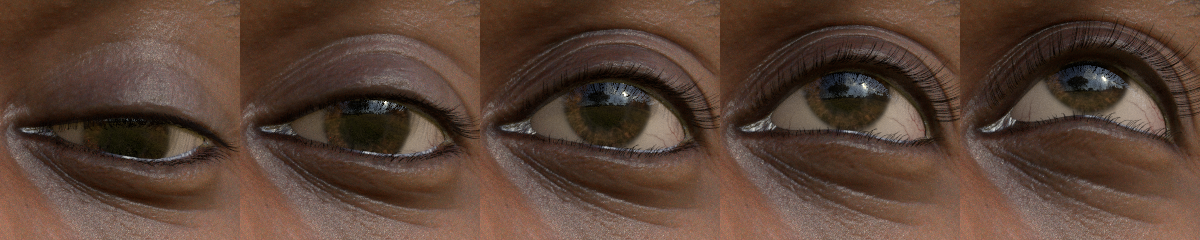
\includegraphics[width=\columnwidth]{eyelid_motion.png}
    \caption{Eyelids are posed by interpolating between blend shapes based on gaze direction. Note how we simulate the folding of the skin above and below the eye.}
    \label{fig:eyelids}
\end{figure}

% Eyelashes are connected to eyelids after all, so I think we can join subsections here.
% \subsection{Modelling of Eyelashes}

\commentY{At least we should give a different subsection title covering both eyelid motion and eyelashes?}
Eyelashes are short curved hairs that grow from the edges of the eyelids.
These can occlude parts of the eye and affect eye tracking algorithms, so are simulated as part of our comprehensive model.
We followed the approach of {\'S}wirski and Dodgson~\cite{swirski2014rendering}, and modelled eyelashes using directed hair particle effects.
Particles were generated from a control surface manually placed below the eyelids.
To make them curl, eyelash particles experienced a slight amount of gravity during growth (negative gravity for the upper eyelash).

\subsection{Eye-Region Landmark Annotation}

\commentY{In my understanding, this section is only related to the shape registration task. And I think some parts in the next section are only relevant to the gaze estimation task? In this case, we should reorganize the next section as a "training data synthesis", starting from a general discussion and task-specific subsections.}

As shown in \autoref{fig:process_ldmks}, each 3D eye-region was annotated once in 3D with $28$ landmarks, corresponding to the eye corners ($2$), eyelids ($5\!+\!5$), iris boundary ($8$), and pupil boundary ($8$).
The iris and pupil landmarks were defined as a subset of the eyeball geometry vertices, so deform automatically with changes in pupil and iris size.
The eyelid and eye corner landmarks were manually labelled with a separate mesh that follows the seam where eyeball geometry meets skin geometry.
This mesh is assigned shape keys and deforms automatically during eyelid motion.
%
% So instead of having humans ambiguously label eye-region anatomy, we carefully manually annotate each eye-region once, ensuring higher-quality labels.
% Maybe put the sentence below in later
Whenever an image is rendered, the 2D image-space coordinates of these 3D landmarks are calculated using the camera projection matrix and saved.
%!TEX root = 00_main.tex

\section{Training Data Synthesis}

\begin{figure}
	\captionsetup[subfigure]{labelformat=empty} % stop subcaption writing "(a)""
    \captionsetup{subrefformat=parens} % add parentheses to \subref
    \centering
    \begin{subfigure}[t]{0.48\columnwidth}
        \inlinelabel{a}{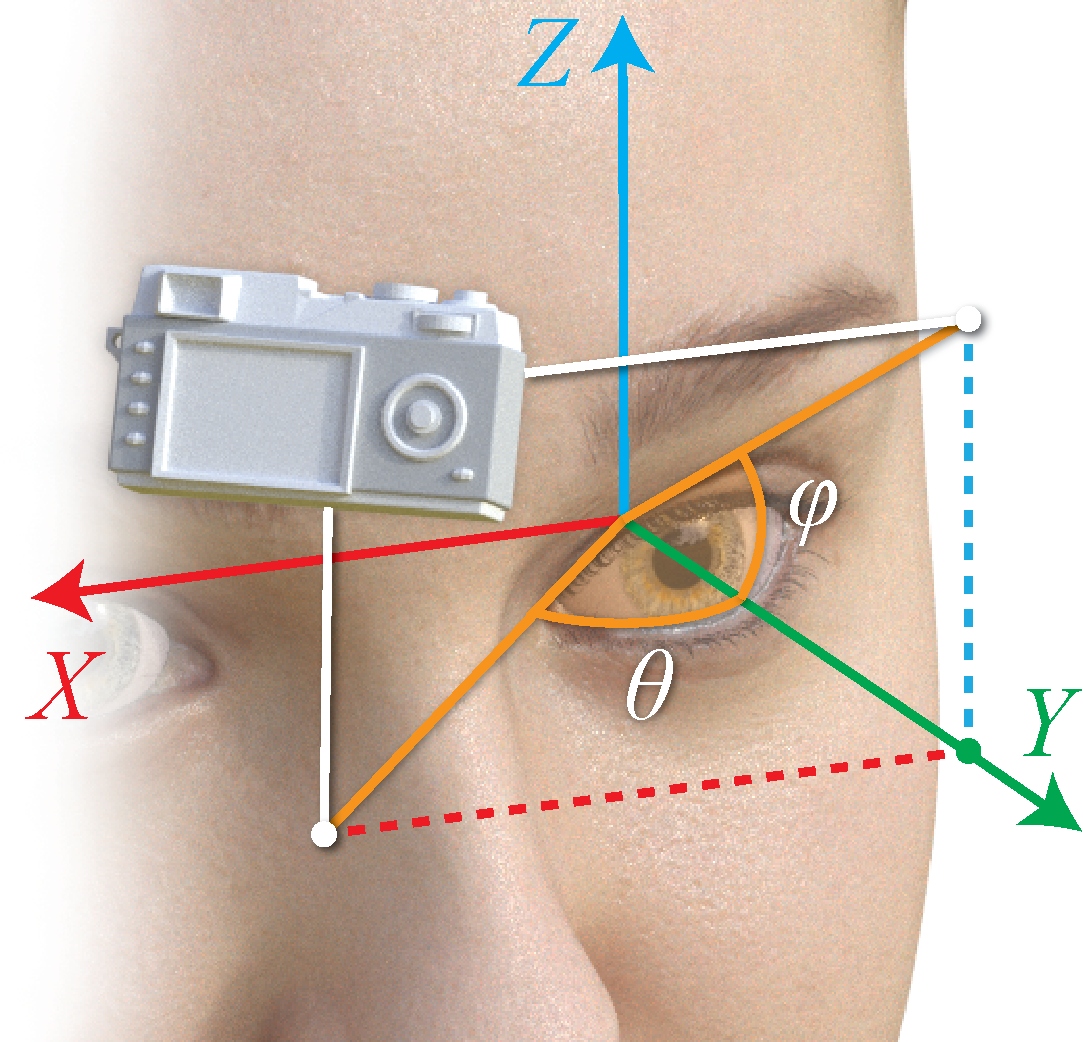
\includegraphics[width=\textwidth]{camera_position}}
        \caption{}\label{fig:cam_pos_spher_coords}
    \end{subfigure}
    \hfill
    \begin{subfigure}[t]{0.48\columnwidth}
        \inlinelabel{b}{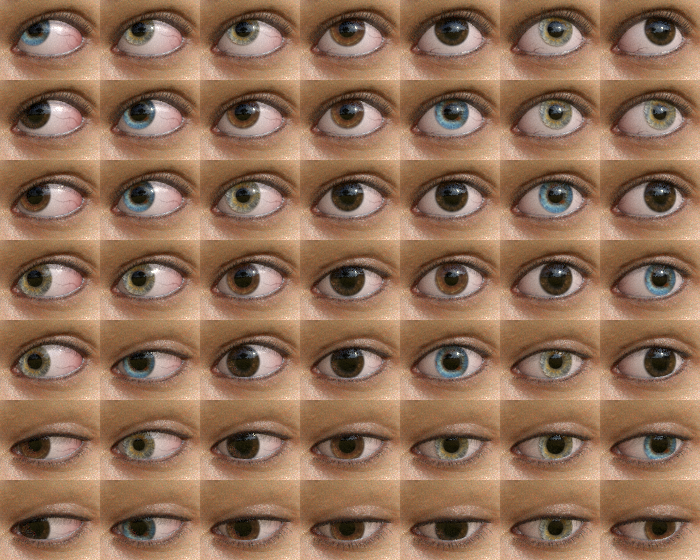
\includegraphics[width=\textwidth]{camera_pos_sample_renders_7x7}}
        \caption{}\label{fig:cam_pos_example_renders}
    \end{subfigure}
    \par\vspace{-28pt}
    \caption{The camera is positioned to simulate changes in head pose \subref{fig:cam_pos_spher_coords}. At each position, we render many eye images for different gaze directions by posing the eyeball model \subref{fig:cam_pos_example_renders}.}
    \label{fig:cam_pos}
\end{figure}

% reword?
In-the-wild images exhibit large amounts of appearance variability across different viewpoints and illuminations.
Our goal was to sufficiently sample our model across these degrees of variation to create representative image datasets.
% \commentY{Did we already clearly state that this paper focuses on these two tasks?}
In this section we first describe how we posed our viewpoint and model, and explain our approach for using image-based lighting \cite{debevec2002image} to model a wide range of realistic environments.
We then describe our landmark annotation process and finally discuss the details of our rendering setup.

\subsection{Posing the Model}

% not sure if its worthwhile trying to formally parameterize the rendering model in the paper
% might be simpler to just use words?
For a chosen eye-region model configuration, each rendered image is determined by parameters $(\mathbf{c}, \mathbf{g}, L)$: 3D camera position $\mathbf{c}$; 3D gaze vector $\mathbf{g}$; and lighting environment $L$.
Camera positions $\mathbf{c}$ were chosen by iterating over spherical coordinates $(r, \theta, \phi)$, centered around the eyeball center (see~\autoref{fig:cam_pos}).
We used orthographic rendering, as this simulates an eye region-of-interest being cropped from a wide-angle camera image, so we set $r\!=\!1$ for convenience.
At each camera position $\mathbf{c}$, we rendered multiple images with different 3D gaze vectors to simulate the eye looking in different directions.
Examples with fixed $L$ are shown in \autoref{fig:cam_pos_example_renders}.
Gaze vectors $\mathbf{g}$ were chosen by first pointing the eye directly at the camera (simulating eye-contact), and then modifying the eyeball's pitch ($\alpha$) and yaw ($\beta$) angles over a chosen range.
For our generic dataset, we rendered images with up to $45^{\circ}$ horizontal and vertical deviation from eye-contact, in increments of $10^{\circ}$.
%
As we posed the model in this way, there was the possibility of rendering ``unhelpful'' images that either simulate impossible scenarios or are not useful for training.
To avoid violating anatomical constraints, we only rendered images for valid eyeball rotations $|\alpha|\!\leq\!25^{\circ}$ and $|\beta|\!\leq\!35^{\circ}$ \cite{MIL-STD-1472G}.
Before rendering, we also verified that the projected 2D pupil center in the image was within the 2D boundary of the eyelid landmarks -- this prevented us from rendering images where too little of the iris was visible.

\subsection{Creating Realistic Illumination}

\begin{figure}
    \begin{subfigure}[t]{\columnwidth}
        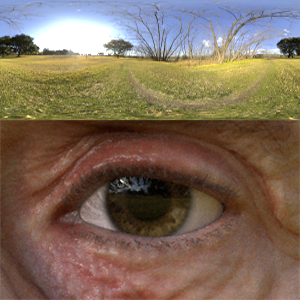
\includegraphics[width=0.24\textwidth]{fig_env_1} \hfill
    	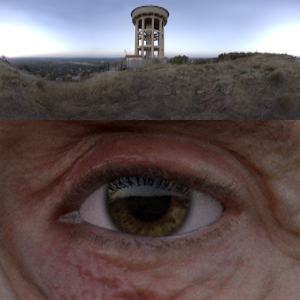
\includegraphics[width=0.24\textwidth]{fig_env_2} \hfill
        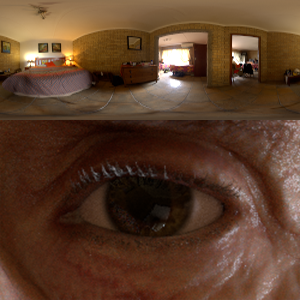
\includegraphics[width=0.24\textwidth]{fig_env_3} \hfill
    	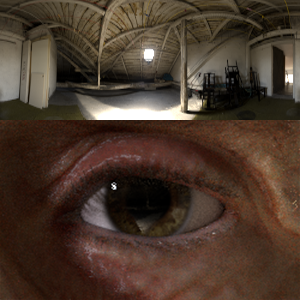
\includegraphics[width=0.24\textwidth]{fig_env_4}
	    \caption{The four HDR environment maps we use for realistic lighting: bright/cloudy outdoors, and bright/dark indoors}
    \end{subfigure}
    \par \medskip
    \begin{subfigure}[t]{0.48\columnwidth}
        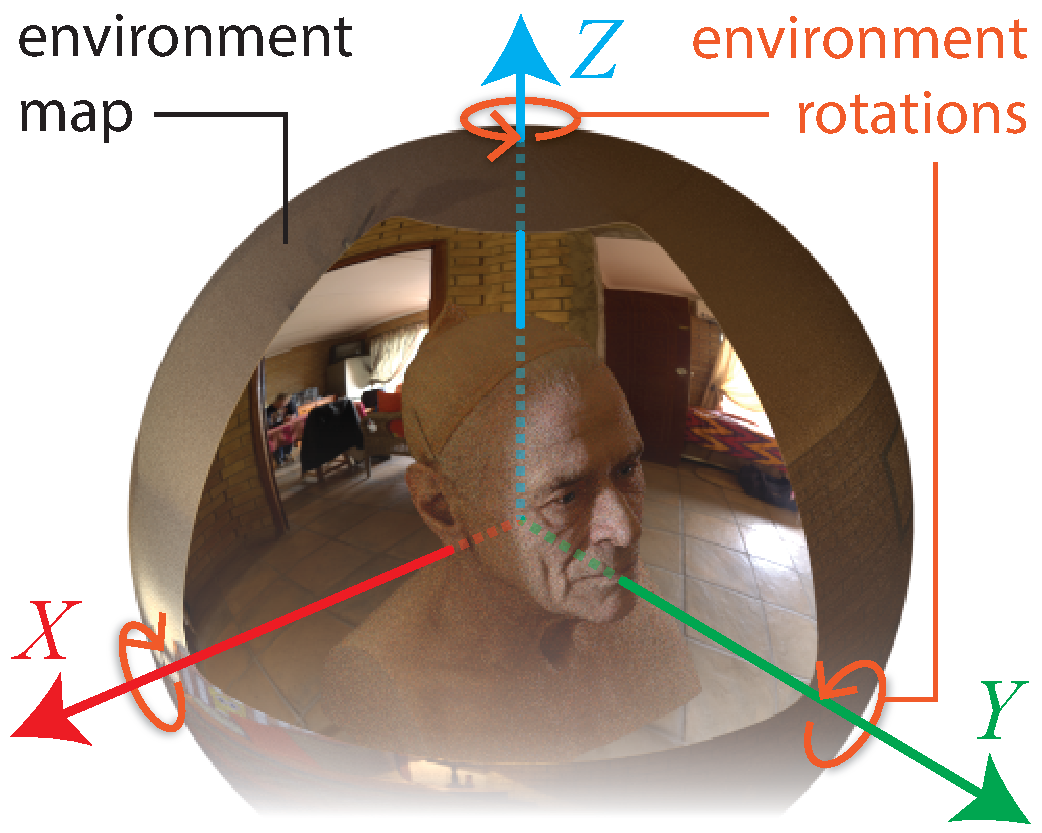
\includegraphics[width=\textwidth]{env_explain_5x4}
    	\caption{The environment is rotated to simulate different head poses}
    \end{subfigure}%
    \hfill
    \begin{subfigure}[t]{0.48\columnwidth}
        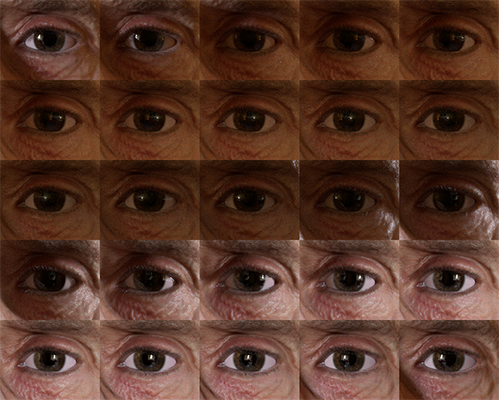
\includegraphics[width=\textwidth]{env_variation}
        \caption{Renders using a single environment, rotated about $Z$}
        \label{fig:env_map_imgs_examples}
    \end{subfigure}
    \caption{Appearance variation from lighting is modelled with poseable high dynamic range environment maps \cite{debevec2002image}.}
    \label{fig:environment_maps}
\end{figure}

One of the main challenges in computer vision is illumination invariance -- a good system should work under a range of real-life lighting conditions.
We realistically illuminate our eye-model using \emph{image-based lighting}, a technique where high dynamic range (HDR) panoramic images are used to provide light in a scene \cite{debevec2002image}.
This works by photographically capturing omni-directional light information, storing it in a texture, and then projecting it onto a sphere around the object.
When a ray hits that texture during rendering, it takes that texture's pixel value as light intensity.
At render time we randomly chose one of four freely available HDR environment images\footnote{\url{http://adaptivesamples.com/category/hdr-panos/}} to simulate a range of different lighting conditions (see \autoref{fig:environment_maps}).
%\cite{AdaptiveSamplesHDR}.
The environment is then randomly rotated to simulate a continuous range of head-pose, and randomly scaled in intensity to simulate changes in ambient light.
As shown in \autoref{fig:env_map_imgs_examples}, a combination of hard shadows and soft light can generate a range of appearances from only a single HDR environment.
% This simple and flexible approach creates variability using measured light levels in real-world environments rather than randomly configuring light sources and ambient illumination \cite{zface}.
% \commentY{We may need a justification (or evidence)}

\subsection{Eye-Region Landmark Annotation}

% \commentY{In my understanding, this section is only related to the shape registration task. And I think some parts in the next section are only relevant to the gaze estimation task? In this case, we should reorganize the next section as a "training data synthesis", starting from a general discussion and task-specific subsections.}
% \commentY{Added a sentence here}
For eye shape registration, we need additional ground-truth annotations of eye-region landmarks in the training images.
As shown in \autoref{fig:process_ldmks}, each 3D eye-region was annotated once in 3D with $28$ landmarks, corresponding to the eye corners ($2$), eyelids ($5\!+\!5$), iris boundary ($8$), and pupil boundary ($8$).
The iris and pupil landmarks were defined as a subset of the eyeball geometry vertices, so deform automatically with changes in pupil and iris size.
The eyelid and eye corner landmarks were manually labelled with a separate mesh that follows the seam where eyeball geometry meets skin geometry.
This mesh is assigned shape keys and deforms automatically during eyelid motion.
%
% So instead of having humans ambiguously label eye-region anatomy, we carefully manually annotate each eye-region once, ensuring higher-quality labels.
% Maybe put the sentence below in later
Whenever an image is rendered, the 2D image-space coordinates of these 3D landmarks are calculated using the camera projection matrix and saved.

\subsection{Rendering Images}

We use Blender's\footnote{The Blender Project -- \url{http://www.blender.org/}} inbuilt Cycles path-tracing engine for rendering.
This Monte Carlo method traces the paths of many light rays per pixel, scattering light stochastically off physically-based materials in the scene until they reach illuminants.
A GPU implementation is available for processing large numbers of rays simultaneously ($150/\textrm{px}$) to achieve noise-free and photorealistic images.

% For eye-region registration \commentY{how about gaze estimation?},
We rendered a generic \dataset dataset of 11,382 images covering $40^{\circ}$ of viewpoint (i.e. head pose) variation and $90^{\circ}$ of gaze variation.
We sampled eye color and environmental lighting randomly for each image.
Each $120\!\times\!80\textrm{px}$ rendering took $5.26\textrm{s}$ on average using a commodity GPU (Nvidia GTX660).
As a result we can specify and render a cleanly-labelled dataset in under a day on a single machine -- a fraction of the time taken by traditional data collection procedures \cite{zhang15_cvpr}.
%!TEX root = 00_main.tex

\section{Experiments}

%\commentA{the distribution figures would be nice here, e.g. to make the point that we can synthesise arbitrary distributions and to beef up the gaze estimation experiments}

% \begin{figure}
%     \centering
%     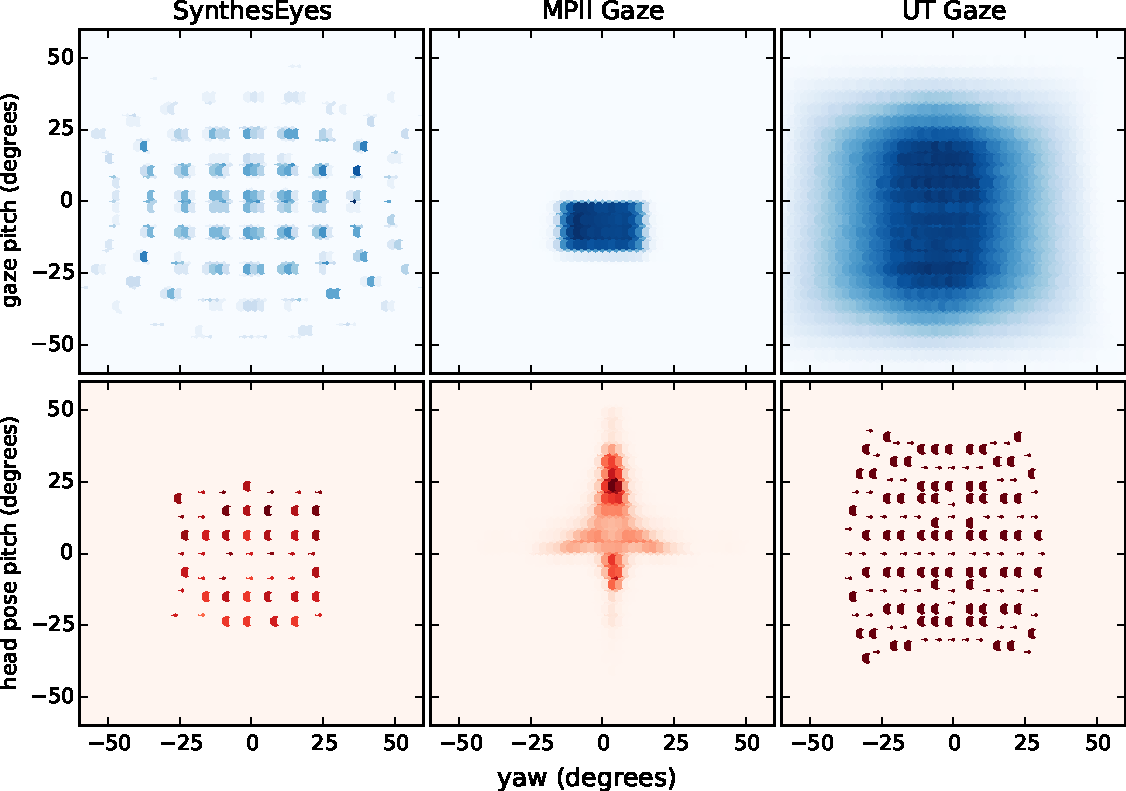
\includegraphics[width=\textwidth]{head_gaze_distribution_v2.pdf}
%     \caption{The head pose (first row) and gaze direction (second row) distribution of different datasets.}
%     \label{fig:head_gaze_distribution}
% \end{figure}

%\commentA{just a reminder to potentially remove the top row in Figure 8 (head pose distributions)}

% \begin{figure}
    \centering
    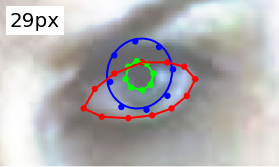
\includegraphics[width=0.244\columnwidth]{figs/wild_ldmks_examples/idx_550.png}\hfill
    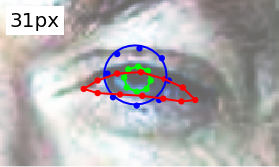
\includegraphics[width=0.244\columnwidth]{figs/wild_ldmks_examples/idx_560.png}\hfill
    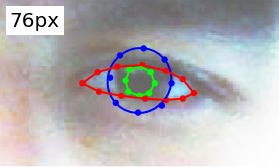
\includegraphics[width=0.244\columnwidth]{figs/wild_ldmks_examples/idx_799.png}\hfill
    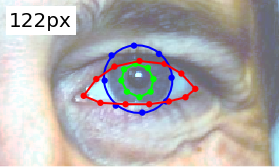
\includegraphics[width=0.244\columnwidth]{figs/wild_ldmks_examples/idx_721.png}
    \par \vspace{0.1em}
    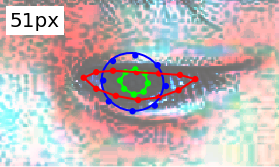
\includegraphics[width=0.244\columnwidth]{figs/wild_ldmks_examples/idx_1013.png}\hfill
    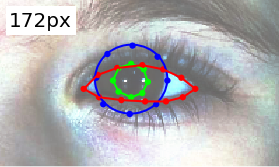
\includegraphics[width=0.244\columnwidth]{figs/wild_ldmks_examples/idx_1002.png}\hfill
    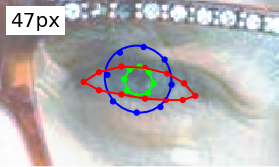
\includegraphics[width=0.244\columnwidth]{figs/wild_ldmks_examples/idx_765.png}\hfill
    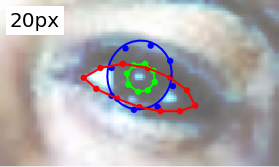
\includegraphics[width=0.244\columnwidth]{figs/wild_ldmks_examples/idx_508.png}
    \par \vspace{0.1em}
    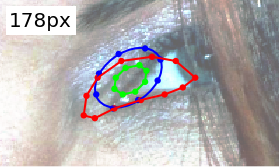
\includegraphics[width=0.244\columnwidth]{figs/wild_ldmks_examples/idx_934.png}\hfill
    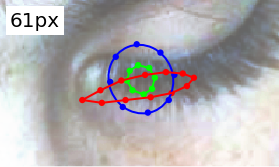
\includegraphics[width=0.244\columnwidth]{figs/wild_ldmks_examples/idx_875.png}\hfill
    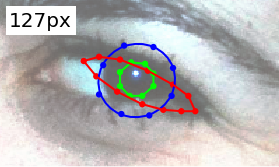
\includegraphics[width=0.244\columnwidth]{figs/wild_ldmks_examples/idx_913.png}\hfill
    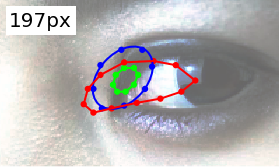
\includegraphics[width=0.244\columnwidth]{figs/wild_ldmks_examples/idx_953.png}
    %
    \caption{The top two rows illustrate successful eye-shape registration on 300-W. The bottom row illustrates failure cases, including un-modelled occlusions and eyelid poses.}
    \label{fig:example_fits_wild}
\end{figure}

% \commentA{briefly say something about significance/importance of both problems, more in corresponding subsections}

\commentY{Maybe this should be presented earlier (in the related works section? we are currently missing references to other appearance-based gaze estimation methods), definition of the two tasks and why and how synthetic data is expected to be helpful. Especially eye-shape registration is not well defined during the previous section}
We evaluated the usefulness of our synthetic data generation method on two sample problems, eye-shape registration and appearance-based gaze estimation.
%
Eye-shape registration attempts to detect biological landmarks of the eye -- eyelids, iris and the pupil. 
Such approaches either attempt to model the shape of the eye directly by relying on edge information \cite{wood2014eyetab, swirski2012robust} or by using statistically learnt deformable models \cite{alabort2014statistically}. 
As our method can reliably generate consistent landmark location training data, we use it for Constrained Local Neural Field (CLNF) \cite{baltrusaitis2013constrained} deformable model training.

\commentY{Edited this paragraph}
Appearance-based gaze estimation systems learn a mapping directly from eye image pixels to gaze direction.
While most of the prior work focused on the {\em person-dependent} training scenario which assumes training data from the target user, recently more attention is paid to the {\em person-independent} training scenario~\cite{funes2013person,schneider2014manifold,sugano2014learning,zhang15_cvpr}. 
% This is in contrast to geometry-based approaches that rely on tracking features of 
%This is a challenging task considering the changes in appearance, 
%thus requiring large amounts of training data to perform well.
The training dataset is required to cover the potential changes in appearance with different eye shapes, arbitrary head poses, gaze directions, and illumination conditions.
%
%Since our method allows the synthesis of eye images with arbitrary head poses, gaze directions, and illumination conditions, we can generate a suitable training dataset rapidly, and even tailor it to the target domain.
Compared to \citet{sugano2014learning}, our method can provide a wider range of illumination conditions which can be beneficial to handle the unknown illumination condition in the target domain.


%\subsection{Eye-Shape Registration In the Wild}

\subsection{Eye-Shape Registration}

\commentY{I feel this subsection + paragraph structure is better to summarize two shape registration experiments?}

\paragraph{Eye-Shape Registration In the Wild}

% \commentA{maybe this should also read eye-shape registration in both section heading and text to be consistent with the next subsection}

\begin{figure}
    \centering
    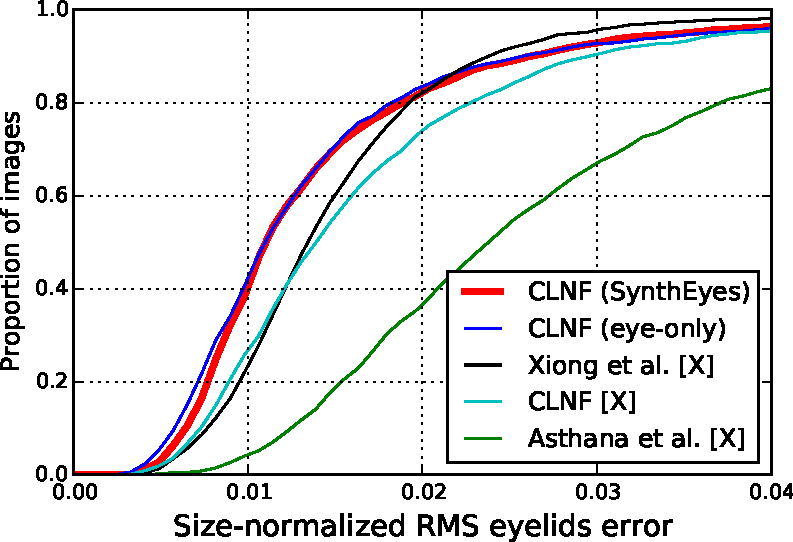
\includegraphics[width=\columnwidth]{figs/CLNF_300W_experiment.pdf}
    \caption{We outperform the state-of-the-art for eyelid-registration in the wild. The right plot shows how performance degrades for training data without important degrees of variation: realistic lighting and eyelid movement.}
    \label{fig:clnf_results_wild}
\end{figure}

% \begin{figure}
    \centering
    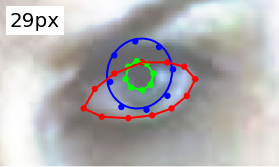
\includegraphics[width=0.244\columnwidth]{figs/wild_ldmks_examples/idx_550.png}\hfill
    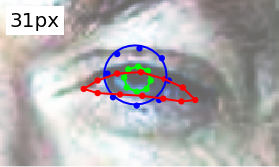
\includegraphics[width=0.244\columnwidth]{figs/wild_ldmks_examples/idx_560.png}\hfill
    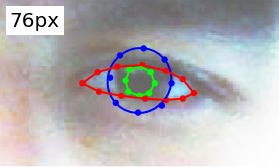
\includegraphics[width=0.244\columnwidth]{figs/wild_ldmks_examples/idx_799.png}\hfill
    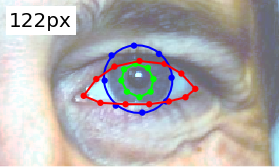
\includegraphics[width=0.244\columnwidth]{figs/wild_ldmks_examples/idx_721.png}
    \par \vspace{0.1em}
    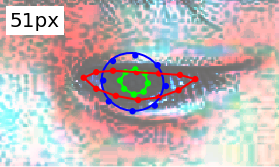
\includegraphics[width=0.244\columnwidth]{figs/wild_ldmks_examples/idx_1013.png}\hfill
    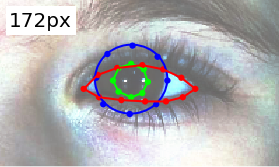
\includegraphics[width=0.244\columnwidth]{figs/wild_ldmks_examples/idx_1002.png}\hfill
    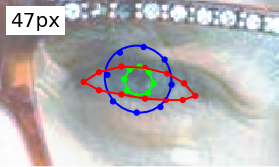
\includegraphics[width=0.244\columnwidth]{figs/wild_ldmks_examples/idx_765.png}\hfill
    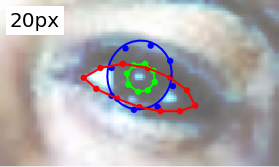
\includegraphics[width=0.244\columnwidth]{figs/wild_ldmks_examples/idx_508.png}
    \par \vspace{0.1em}
    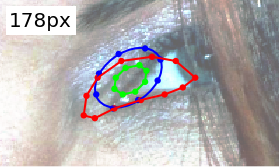
\includegraphics[width=0.244\columnwidth]{figs/wild_ldmks_examples/idx_934.png}\hfill
    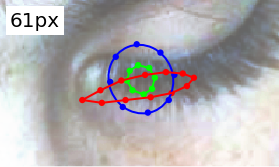
\includegraphics[width=0.244\columnwidth]{figs/wild_ldmks_examples/idx_875.png}\hfill
    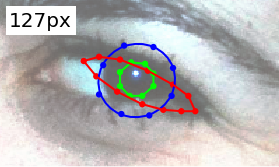
\includegraphics[width=0.244\columnwidth]{figs/wild_ldmks_examples/idx_913.png}\hfill
    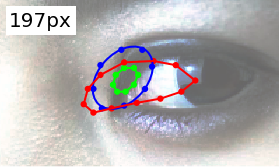
\includegraphics[width=0.244\columnwidth]{figs/wild_ldmks_examples/idx_953.png}
    %
    \caption{The top two rows illustrate successful eye-shape registration on 300-W. The bottom row illustrates failure cases, including un-modelled occlusions and eyelid poses.}
    \label{fig:example_fits_wild}
\end{figure}

% Erroll to Tadas: need to make sure these facts are straight...
We performed an experiment to see how our our system generalises on unseen and unconstrained images from the 300 Faces In-the-Wild (300-W) challenge \cite{sagonas2013300} validation datasets which contain labels for eyelid boundaries. We tested all of the approaches on the 830 (out of 1026) test images. We discarded images that did not contain visible eyes (occluded by hair or sunglasses) or where face detection failed in some of the baselines. This lead to 1660 eye images for evaluation.

We trained CLNF patch experts using the generic \dataset dataset and used the 3D landmark locations to construct a Point Distribution Model (PDM) using Principal Component Analysis. 
As our rendered images did not contain closed eyes we generated extra closed eye landmark labels by moving the upper eyelid down to lower one or meeting both eyelids halfway.
We initialised our approach by using the face-CLNF \cite{baltrusaitis2013constrained} facial landmark detector.

To compare using synthetic or real training images, we trained an eyelid CLNF model on 300-W images, but used the same PDM used for synthetic data (CLNF 300-W).
We also compared our approach with the following state-of-the-art facial landmark detectors trained on real world in-the-wild data: CLNF \cite{baltrusaitis2013constrained}, Supervised Descent Method (SDM) \cite{Xiong2013sdm}, Discriminative Response Map Fitting (DRMF) \cite{Asthana2013drmf}, and tree based face and landmark detector \cite{Zhu2012tree}. 

The results of our experiments can be seen in \autoref{fig:clnf_results_wild}, and example model fits are shown in \autoref{fig:fits_300W}.
Errors were recorded as the RMS point-to-boundary distance from tracked eyelid landmarks to ground truth eyelid boundary, and were normalized by inter-ocular distance. 
First, the results show the eye-CLNF (both synthetic ($\mathrm{Mdn}=0.0110$) and real data ($\mathrm{Mdn}=0.0110$) outperforming all other systems in eye-lid localization: SDM ($\mathrm{Mdn}=0.0134$), face-CLNF ($\mathrm{Mdn}=0.0139$), DRMF ($\mathrm{Mdn}=0.0238$), and Tree based ($\mathrm{Mdn}=0.0217$). 
Second, our system (CLNF Synth) trained on only ten participants in four lighting conditions results in very similar performance to a system trained on unconstrained in-the-wild images (CLNF 300-W). This suggests the importance of high-quality consistent labels.
% and that our system can be used to achieve state-of-the-art performance for eye shape registration. 
%Furthermore, our approach managed to generalise without explicit modelling of eye-glasses or other partial occlusions.

Our data synthesis system also allows us to examine what steps of the synthesis approach are important for generating good training data. We trained two further eye-CLNFs on different versions of \dataset, one without eyelid motion and one with only one fixed lighting condition. As can be seen in \autoref{fig:clnf_results_wild}, not using shape variation ($\mathrm{Mdn}=0.0129$) and using basic lighting ($\mathrm{Mdn}=0.0120$) leads to worse performance due to missing degrees of variability.

%\subsection{Eye-Shape Registration for Webcams}
\paragraph{Eye-Shape Registration for Webcams}

% \commentA{``for laptops'' sounds very specific. Does this generalise, do we need this strong constraint?}

%!TEX root = ../00_main.tex

%
\begin{figure*}[ht]
    \captionsetup[subfigure]{labelformat=empty} % stop subcaption writing "(a)""
    \captionsetup{subrefformat=parens} % add parentheses to \subref
    \centering
    \begin{subfigure}[t]{\columnwidth}
        \inlinelabel{a}{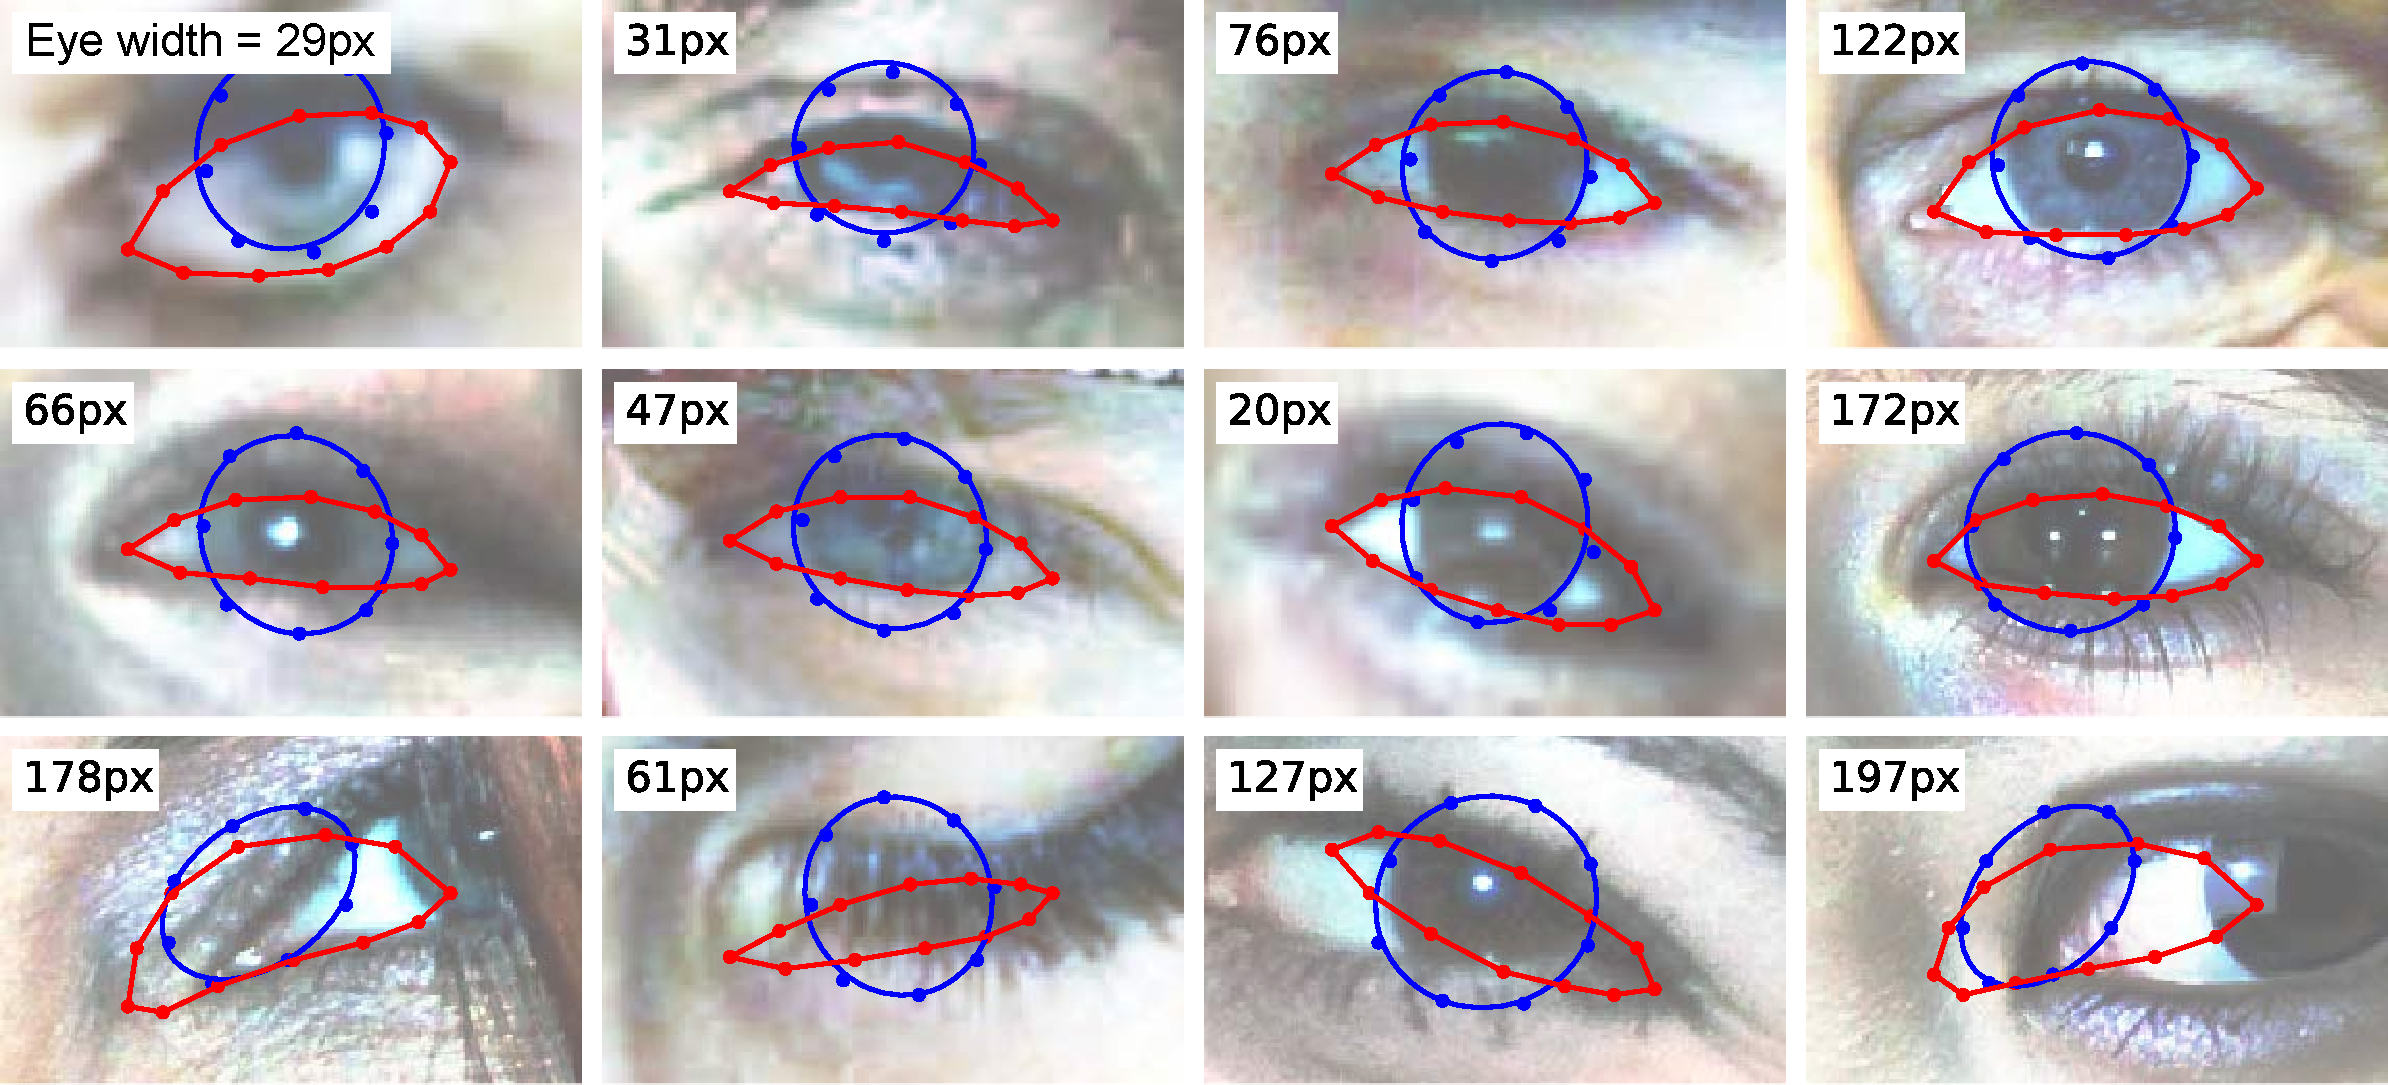
\includegraphics[width=\textwidth]{fits_300W}}
        \caption{}\label{fig:fits_300W}
    \end{subfigure}
    \hfill
    \begin{subfigure}[t]{\columnwidth}
        \inlinelabel{b}{\includegraphics[width=\textwidth]{fits_MPII}}
        \caption{}\label{fig:fits_MPII}
    \end{subfigure}
    \par\vspace{-28pt}
    \caption{Example fits of our eye-CLNF trained on \dataset on in-the-wild images \subref{fig:fits_300W} and webcam images \subref{fig:fits_MPII}. The top two rows illustrate successful eye-shape registration, while the bottom rows illustrate failure cases, including unmodelled occulsions (hair), unmodelled poses (fully closed eye), glasses, and incorrect model initializaion.}
    \label{fig:example_fits}
\end{figure*}

\begin{figure}
    \centering
    \includegraphics[width=\columnwidth]{CLNF_MPII_experiment}
    \caption{We perform comparably with state-of-the-art for iris-registration on in-the-wild webcam images.}
    \label{fig:clnf_results_MPII}
\end{figure}

While the 300-W images represent challenging conditions for eyelid registration, they are not representative of typical webcam-style images and do not feature iris labels.
We therefore annotated sub-pixel eyelid and iris boundaries onto a subset of MPIIGaze (188 images), a recent large-scale dataset of face images and corresponding on-screen gaze locations collected during everyday laptop use over several months \cite{zhang15_cvpr}.
Pupil accuracy was not evaluated as it was impossible to discern in in most images.
We compared our eye-CLNF with EyeTab \cite{wood2014eyetab}, a state-of-the-art shape-based approach for webcam gaze estimation that robustly fits ellipses to the iris boundary using image-aware RANSAC \cite{swirski2012robust}.
We used a modified version of the author's implementation with improved eyelid localization using CLNF \cite{baltrusaitis2013constrained}.
As a baseline, we used the mean position of all 28 eye-landmarks following model initialization.
Eyelid errors were calculated as RMS distances from eyelid landmarks to the ground truth eyelid boudnary.
Iris errors were calculated by first least-squares fitting an ellipse to the tracked iris landmarks, discretizing it, removing points outside ground truth and tracked eyelid boundaries, and then measuring RMS distances to the ground truth iris.
This avoided calculating errors for parts of the iris which were occluded by the eyelid.
Errors were normalized by the eye-width, and are reported using average eye-width ($44.4\textrm{px}$) as reference.

As shown in \autoref{fig:clnf_results_MPII}, our approach ($\textrm{Mdn}\!=\!1.48\textrm{px}$) demonstrates comparable iris-fitting accuracy with EyeTab ($\textrm{Mdn}\!=\!1.44\textrm{px}$), a state-of-the-art algorithm for fitting ellipses to irises in low-quality images.
However, our eye-CLNF is more robust, with EyeTab failing to terminate in $2\%$ of test cases.
As also shown by the 300-W experiment, our eye-CLNF localizes eyelids better than the face-CLNF.
See \autoref{fig:fits_MPII} for example model fits.
%As shown by \todo{prev exp.}, our eye-CLM ($2.79\!\pm\!2.20\textrm{px}$) also localizes eyelids better than previous state-of-the-art facial landmark trackers ($4.27\!\pm\!1.84\textrm{px}$).

% show that we only need data from few(er) people and show competitive performance
% Maybe) Plot landmark accuracy on LFW against number of training participants. Show that even with just a few participants (e.g. 4) we get good results for eyelid positions compared to state-of-the-art face trackers.

% eye corner detection
% eye bounding box detection
% eye position detection?
% ^ I think all of these come with what the deformable model gives us

\subsection{Appearance-Based Gaze Estimation}

% evaluate eye/gaze/eyelid shapes (fully synthetic) separately from full face appearance (which is a mixture of real and synthetic data)

% person-adaptation, use pre-trained model from synthesised data, then personalise with small amount of user-specific data
% ^ let's leave this as future work! Can put it in the discussion 

% show that we can synthesise specific datasets for specific settings (specific head and gaze ranges, illumination conditions), show that we can competitive performance

\begin{figure}
    \centering
    \includegraphics[width=\columnwidth]{head_gaze_distribution_v2.pdf}
    \caption{The gaze direction (first row, blue) and head pose (second row, red) distributions of different datasets.}
    \label{fig:head_gaze_distribution}
\end{figure}

\begin{figure}
    \centering
    \includegraphics[width=\columnwidth]{gazeResult.pdf}
    \caption{Gaze estimation performance comparison. The X axis indicates the test set is the MPIIGaze dataset or its frontal pose subset. The legend shows different training sets.}
    \label{fig:gazeResult}
\end{figure}

\commentY{Edited this paragraph}
To evaluate the usage of our method on appearance gaze estimation, we perform the cross-dataset validation as described in \citet{zhang15_cvpr}, where they train and test the model on different datasets. 
We synthesized our dataset using the same camera setting as UT dataset~\cite{sugano2014learning}, and the same normalization scheme can be applied to the test data.
The training data is fully compatible with UT dataset, and we can directly compare our~\dataset using the same Convolutional Neural Network (CNN) model~\cite{zhang15_cvpr}.

%Following the same setting, we train the same Convolutional Neural Network (CNN) model on the generic~\dataset dataset, and test it on MPIIGaze evaluation subset proposed by~\cite{zhang15_cvpr}. 
As shown with the two bars at the far left of~\autoref{fig:gazeResult}, compared to the mean gaze direction prediction error 13.9 degrees that trained with UT dataset, the model trained with our generic~\dataset dataset can achieve the same performance with 14.0 degrees mean error. It confirms that our method can generate a equivalent data for the appearance-based gaze estimation training.
\commentY{Moved \& edited}
The fifth bar of~\autoref{fig:gazeResult} shows the leave-one-person-out cross validation within the MPIIGaze dataset to show the up bounder of this scenario.
These result indicates that both \dataset~and UT datasets still have their own error sources which is causing the performance gap.

%\paragraph{Head Pose and Gaze Ranges}
\commentY{Edited}
One of the important factors related to the above gap is the head pose and gaze ranges.
While it is important to cover a wide range of head poses to handle arbitrary camera settings, this can make the training task more difficult.
If the target setting can be preliminary specified, as the laptop interaction case in \citet{zhang15_cvpr}, it is practically possible to limit the synthesis of training data with minimum required head pose and gaze ranges.
%The head pose and gaze direction range are also quite important priors for appearance-based gaze estimation. 
%Since the samples from the small range of head poses can be trained together, while extreme head poses wouldn't share eye appearance. Also the gaze direction space is arbitrary and difficult to be densely covered by collected dataset.
In order to analyze the effect of different head pose ranges, we additionally render a~\dataset subset that matches the gaze and pose distribution of MPIIGaze dataset.
Since our method also allows us to control lighting conditions, we also added 3D laptop screen emitting light to simulate the target condition.
%Notice that the head pose and gaze direction range can be estimated based on the task, so the required information is not sophisticated. 
%This shows how we can target specific scenarios like laptop-based gaze estimation, and render a suitable dataset within a day rather than taking 3 months of data collection with 15 participants. 
For comparison, we also re-sample a subset of UT dataset as described in~\cite{zhang15_cvpr} that has the same gaze and head pose distribution with MPIIGaze.
The head pose and gaze direction distribution are shown in~\autoref{fig:head_gaze_distribution}.

Another important difference between two datasets is the number of subjects in the dataset.
%Since there are just have 10 subjects in our~\dataset, 
In order to compare two approaches with the same number of subjects, we divide the UT Multiview subset into 5 groups with 10 subjects.
Each group of this UT subset has 15,000 samples as with our~\dataset subset.
We then average the performance of the 5 groups for the final result. 
As shown in the third and forth bars of~\autoref{fig:gazeResult}, in general having the similar head pose and gaze direction ranges of target domain can significantly improve the performance. 
\commentY{Put actual numbers here} 
Since both UT subset and~\dataset subset have the similar head pose and gaze direction range, the performance gains should come from the realistic samples generate from precise 3D eye model and also simulated variant appearance caused by light conditions.
This result indicates, under the condition with the same number of face variations, our~\dataset subset can be a better training set compared to UT subset.

\paragraph{Difference Between Synthesis and Realistic Data}
The UT dataset is synthetically generated based on collected data, while our~\dataset is purely synthesis, the different affect between them for the gaze estimation training is interesting. We thus based on the the above experiments to play around their roles in such cross datasets scenario.
We use the pre-trained model on the~\dataset and fine tune it with the UT dataset to test on MPIIGaze dataset, it is the case that we can pre-train the model with the synthetic~\dataset and fine tune the model if we have more realistic data. For caparison, we test the opposite way, i.e. pre-train the model in UT dataset and fine tune it with the~\dataset. As shown in~\autoref{tab:Synthesis_Realistic_Gaze}, our~\dataset is suitable as training data due to its generality while UT doesn't have such quality. 

\begin{table}
\begin{center}
\begin{tabular}{ |c|p{80pt}|p{80pt}| } 
 \hline
 Train set & pre-train~\dataset and fine tune with UT & pre-train UT and fine tune with~\dataset \\ 
 \hline
 Full & X.X & X.X \\ 
 \hline
 Subset & 7.8 & 8.8 \\ 
 \hline
\end{tabular}
\caption{The difference of pre-training on different dataset. The first row show we use the full~\dataset and full UT; The second row show the experiment done with~\dataset subset and UT subset.} 
\label{tab:Synthesis_Realistic_Gaze}
\end{center}
\end{table}


\paragraph{Person Specific Appearance}
Besides head pose and gaze direction ranges, it is well known that person-dependent is always the essayist scenario for gaze estimation, since the similar appearance would make the task much easier. To avoid the tedious personal calibration or long term personal data collection, one option is to use the most similar personal appearance from the training data for testing on target person. However, such training samples selection is limited inside the collected training data. Our method could generate any kind of personal appearance and do not have such limitation. As shown in~\autoref{tab:personal_specific}, there are some subjects that suitable as training set for the MPIIGaze dataset, such as subject 1, 2, 6, 8 and 10. We use these subjects as the training set and can achieve X.X degrees on the MPIIGaze dataset.


\begin{table}
\begin{center}
\begin{tabular}{ |c|c|c|c|c|c| } 
 \hline
 Subject ID & 1 & 2 & 3 & 4& 5 \\ 
 \hline
 Error & 8.5 & 9.0 & 11.65 & 10.72 & 9.3 \\ 
 \hline
 \hline
 Subject ID & 6 & 7 & 8 & 9 & 10 \\ 
 \hline
 Error & 8.3 & 10.4 & 8.5 & 11.1 & 8.6 \\ 
 \hline
\end{tabular}
\caption{The test results on MPIIGaze dataset with the training on individual subjects from~\dataset}
\label{tab:personal_specific}
\end{center}
\end{table}

% \paragraph{Realism and Light Conditions}
% To test the influence of realism and light condition factors, we use the subsets of those datasets that just include frontal face clusters. We first randomly select 10 subjects from UT dataset, and take the frontal pose with their 160 gaze directions as UT frontal subset. Then we generate a~\dataset frontal subset that has the same head pose and gaze distribution with the UT frontal subset in three setting: with varying light conditions, without varying light conditions and without eyelid movement. The test set is the samples in MPIIGaze with head pose within $\pm$ 5 degrees of frontal head pose. The results are shown in~\autoref{tab:frontal_160}.

% \begin{table}
% \begin{center}
% \begin{tabular}{ |c|c| } 
%  \hline
%  Train Set & Estimation Error \\ 
%  \hline
%  SynthEye with varying light condition & 6.8 \\ 
%  \hline
%  SynthEye without varying light condition & 6.7 \\ 
%  \hline
%  SynthEye without eyelid movement & 6.8 \\
%  \hline
% \end{tabular}
% \caption{Result on realism and light conditions}
% \label{tab:frontal_160}
% \end{center}
% \end{table}

% train on synthesised images and show competitive performance on MPIIgaze with real images
% show better performance than UT dataset
%Using Xucong's CNN sytem, we train on targeted version of \dataset, test on MPII. Show results are better than training on UT and testing on MPII. This shows that the range of lighting in \dataset is important for better results.

% does photorealistic data really help/is it necessary? either reduce quality and see how it affects performance, or compare model with and without shape variations
% ^ I am not really sure how to do this well... Because we'd also have to have a measure of "how photorealistic" something is. Swapping the eyeball for a simpler model, e.g. sphere might not really have that much of an effect on "photorealism" for many eye-poses. Changing the shaders, e.g. pretending the skin is Lambertian (diffuse) might?

\commentY{Reminder: ideally we should have a discussion on potential limitations of the current approach}


%!TEX root = 00_main.tex

\section{Conclusion}


% \clearpage

{\small
\bibliographystyle{IEEEtranN}
\bibliography{bib}
}

\end{document}
